%
% FreeBSD 10.1-RELEASE Installation Guide
% (C) 2009-2014 Manolis Kiagias
% Published under the Creative Commons license
%
%!TEX TS-program = xelatex
%!TEX encoding = UTF-8 Unicode
%
\documentclass[a4paper,twoside,12pt]{article}
\usepackage{fontspec,xltxtra,xunicode}
% Begin new paragraphs with an empty line rather than an indent
\usepackage[parfill]{parskip}
%\usepackage{xgreek}
\usepackage{multirow}
\usepackage{longtable}
\usepackage[colorlinks=true,linkcolor=black]{hyperref}
\defaultfontfeatures{Mapping=tex-text}
\setromanfont[Mapping=tex-text]{Times New Roman}
\setsansfont[Scale=MatchLowercase,Mapping=tex-text]{Liberation Sans}
\setmonofont[Scale=MatchLowercase]{Liberation Mono}
\setmainfont[Scale=MatchLowercase]{Liberation Serif}
\usepackage{multicol}
\usepackage{graphicx}
\setcounter{secnumdepth}{4}
\setcounter{tocdepth}{4}
\usepackage{fancyhdr}
\pagestyle{fancy}
\renewcommand{\sectionmark}[1]{%
	\markboth{#1}{}}
\fancyhf{}
\fancyhead[LE,RO]{\bfseries\thepage}
\fancyhead[LO]{\bfseries\rightmark}
\fancyhead[RE]{\bfseries\leftmark}
\renewcommand{\headrulewidth}{0.5pt}
\renewcommand{\footrulewidth}{0pt}
\addtolength{\headheight}{0.5pt}
\fancypagestyle{plain}{%
	\fancyhead{}
	\renewcommand{\headrulewidth}{0pt}}
%
% User defined environments and commands
%
\newenvironment{inthebox}{\line(1,0){390}\\}%
{\line(1,0){390}}
\newcommand{\coderoot}[1]{\texttt{\# #1}}
\newcommand{\codeuser}[1]{\texttt{\$ #1}}
\newcommand{\code}[1]{\texttt{#1}}
%
% Title page
%
\author{Manolis Kiagias, MSc}
\title {FreeBSD 10.1-RELEASE: Base system to Desktop Environment}
\date{01/06/2014}
%
%
\begin{document}
%
\maketitle
\begin{center}

\includegraphics[width=0.95\textwidth]{images/main/freebsd-xorg-logo.png}
\end{center}
%
\cleardoublepage
%
%
% Book intro pages (frontmatter)
%
\begin{center}
Copyright \copyright 2009 -- 2014 Manolis Kiagias

This Work is Provided Under the Terms of the License:\\

\includegraphics[scale=0.2]{images/license/cc-logo}\\
\textbf{Attribution-NonCommercial-ShareAlike 4.0 International}\\
The complete text of this license is available here:\\
\url{http://creativecommons.org/licenses/by-nc-sa/4.0/}
\end{center}
\subsection*{You are free to:}

\noindent
\textbf{Share} -- copy and redistribute the material in any medium or format
\textbf{Adapt} -- remix, transform, and build upon the material

The licensor cannot revoke these freedoms as long as you follow the license terms.

\subsection*{Under the following terms:}

\vspace{1em}
\noindent
\parbox{1.5cm}{
\includegraphics[scale=1.5]{images/license/cc_by_30}}
\parbox{10.5cm}{\textbf{Attribution} — You must give \textbf{approprate credit} provide a link to license, and \textbf{indicate if changes were made}. You may do so in any reasonable manner, but not in any way that suggests the licensor endorses you or your use.}

\vspace{1em}
\noindent
\parbox{1.5cm}{
\includegraphics[scale=1.5]{images/license/cc_nc_30}}
\parbox{10.5cm}{\textbf{NonCommercial} --  You may not use the material for \textbf{commercial purposes}.}

\vspace{1em}
\noindent
\parbox{1.5cm}{
\includegraphics[scale=1.5]{images/license/cc_sa_30}}
\parbox{10.5cm}{\textbf{ShareAlike}  -- If you remix, transform, or build upon the material, you must distribute your contributions under the \textbf{same license} as the original.}

\vspace{1em}
\noindent
\parbox{10.5cm}{\textbf{No additional restrictions} -- You may not apply legal terms or \textbf{technological measures} that legally restrict other from doing anything the license permits.

\subsection*{Notices:}

\noindent
You do not have to comply with the license for elements of the material in the public domain or where your use is permitted by an applicable \textbf{exception or limitation}.

\vspace{1em}
\noindent
No warranties are given. The license may not give you all the permissions necessary for your intended use. For example, other rights such as \textbf{publicity, privacy, or moral rights} may limit how you use the material.
\line(1,0){390}\\\\
\newpage
\tableofcontents
\newpage

%
\section{Installing FreeBSD 10.0-RELEASE}
%
Before beginning any installation of an operating system, we must adjust the BIOS to boot from the intended installation media. Most of the newer PC hardware have the ability to boot off USB devices such as flash drives. In our example installation we will assume a standard CD-based install.

FreeBSD comes in many different versions for 32 and 64bit PC architectures as well as many others. Typically, the 32bit version is used for systems utilizing a Pentium IV or lower grade CPU and the 64bit version for more modern processors such as the Core2/Core4 and newer families.

While FreeBSD is available both on CD and DVD, the DVD version is not required for our install. The additional components in the DVD are ready-made packages that are also available online.

Booting off the installation media, after a while, the first installation dialog appears:

\begin{center}
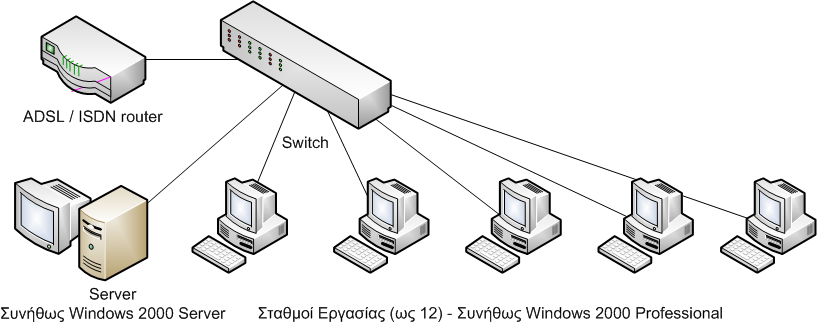
\includegraphics[width=0.95\textwidth]{images/main/school-lab}
\end{center}

Just press Enter on the default Install option.

\begin{center}
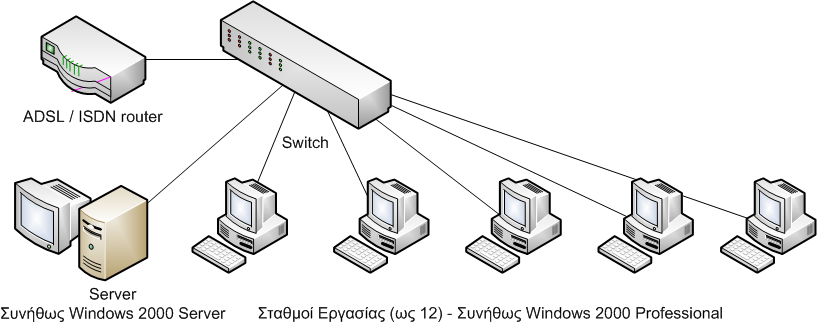
\includegraphics[width=0.95\textwidth]{images/main/school-lab}
\end{center}

Select the desired keyboard layout. This is not a critical setting for a desktop system as it will not affect your GUI settings. If you cannot find the a layout that matches your keyboard/language, just select the US layout.

During the installation process, use the arrow keys to move between options. Use the SPACE bar to mark any checkboxes. Move between different dialog parts using the TAB button.

\begin{center}
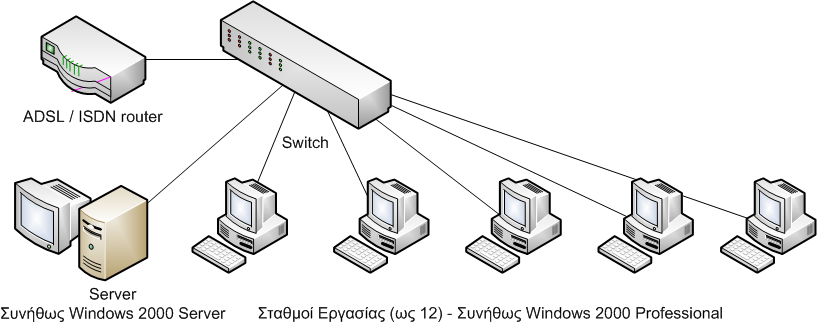
\includegraphics[width=0.95\textwidth]{images/main/school-lab}
\end{center}

After selecting the keyboard layout, just press ENTER on this dialog to confirm it.

\begin{center}
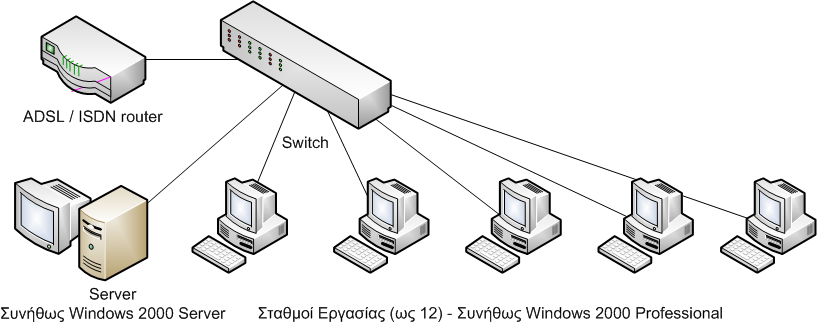
\includegraphics[width=0.95\textwidth]{images/main/school-lab}
\end{center}

Every system must have a hostname. Typically, a system also belongs to a domain. As our system is not directly connected to the Internet (most probably is served by a home DSL router) we may choose any domain name. In our example, the domain name is \textbf{thelab.local} and the hostname is \textbf{beastiebox}. You may come with an original hostname for your system (plants, planets, trees and animals are commonly used) or simply use something as dull as system01.

\begin{center}
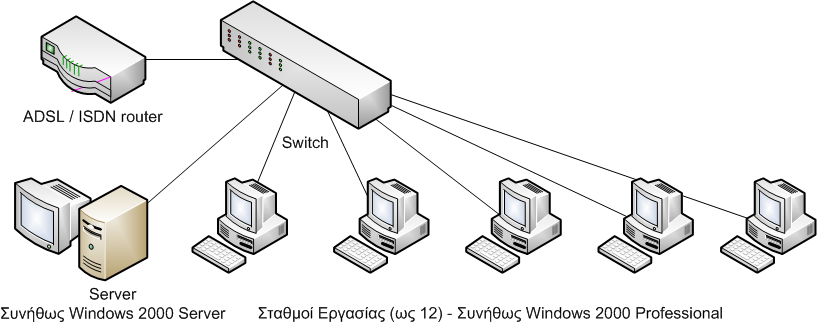
\includegraphics[width=0.95\textwidth]{images/main/school-lab}
\end{center}

In this dialog we select the additional or optional components to install. There is no need to select the Ports tree as the version on the CD is outdated and the ports can be readily installed off the Internet. The system source code is useful as a reference and if you plan to build your own kernel.

\begin{center}
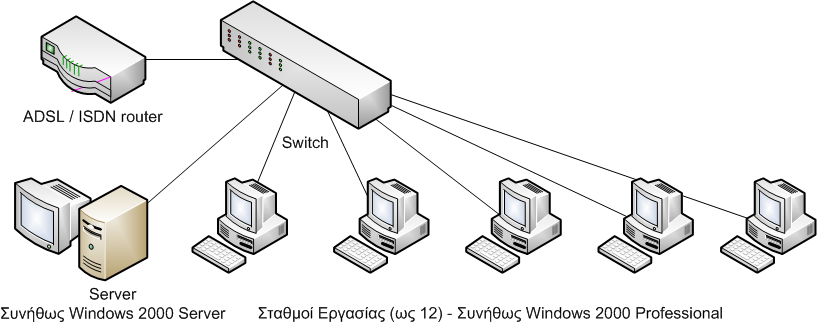
\includegraphics[width=0.95\textwidth]{images/main/school-lab}
\end{center}

Here we select between different ways to partition our disk. The easiest method is to use the default Guided way.

\begin{center}
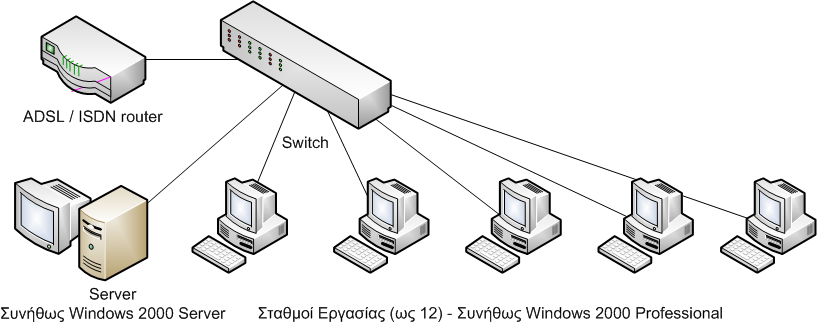
\includegraphics[width=0.95\textwidth]{images/main/school-lab}
\end{center}

In our example we assume a completely empty disk and select the \textbf{Entire Disk} option. Note that this will \textbf{erase} anything on the disk and create appropriate BSD partitions! Multi boot systems may be created by using the \textbf{Partition} option, but this is outside the scope of this concise guide.

\begin{center}
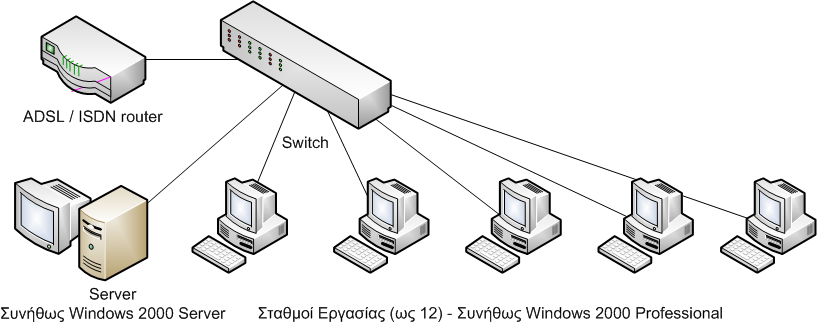
\includegraphics[width=0.95\textwidth]{images/main/school-lab}
\end{center}

Depending on the disk and RAM size of our system, the installation program will suggest different partition sizes. We can usually accept the default settings. Using the options in this dialog we can customize the sizes or create additional partitions. One possible change is to shrink the size of the root partition (marked as ``/'') and create a separate partition for \textbf{/home}. In our sample installation we simply select \textbf{Finish}.

\begin{center}
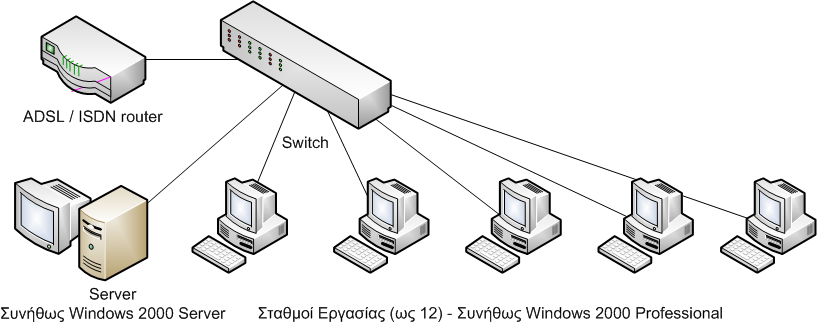
\includegraphics[width=0.95\textwidth]{images/main/school-lab}
\end{center}

This is the final warning: After selecting \textbf{Commit}, our changes will be written to disk, partitions will be created and formatted and files will be copied. Any existing data on the disk will be lost after pressing Commit.

\begin{center}
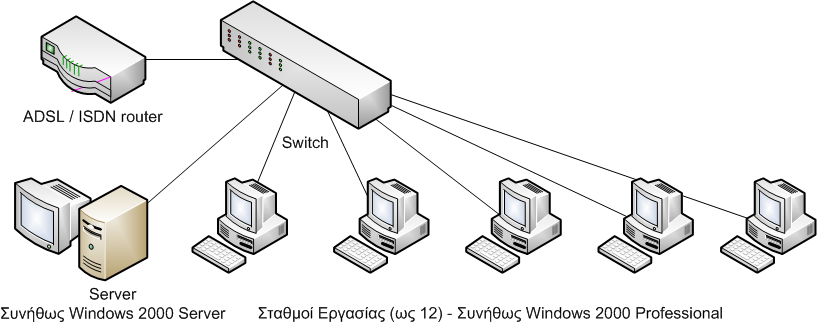
\includegraphics[width=0.95\textwidth]{images/main/school-lab}
\end{center}

File copying will take a while.

\begin{center}
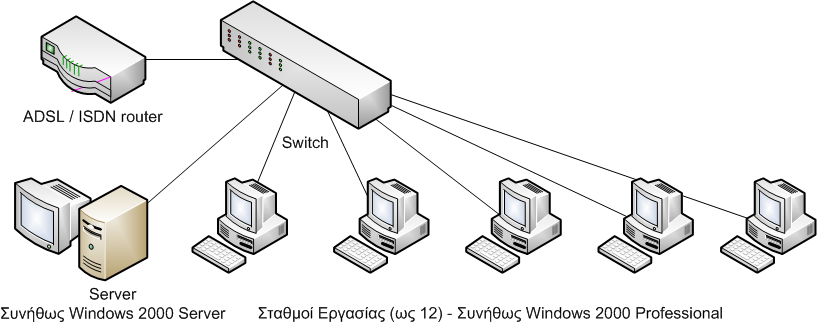
\includegraphics[width=0.95\textwidth]{images/main/school-lab}
\end{center}

We must now set the password for root (admin) user. Use a safe, long password that may not be guessed. You birthday, phone number and 1234 are all unsafe passwords!

\begin{center}
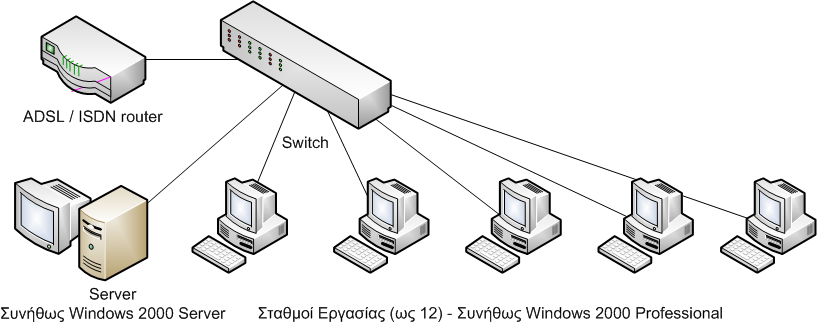
\includegraphics[width=0.95\textwidth]{images/main/school-lab}
\end{center}

The above dialog will appear if the installation program detects a network card. If more than one network cards are detected, their models will be listed here allowing us to choose which one to configure.

\begin{center}
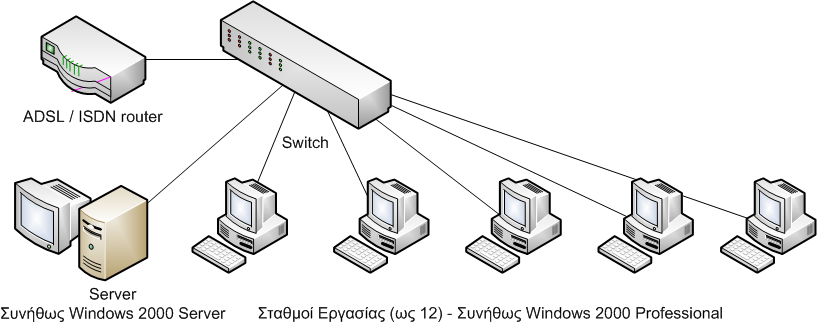
\includegraphics[width=0.95\textwidth]{images/main/school-lab}
\end{center}

The obvious answer is Yes.

\begin{center}
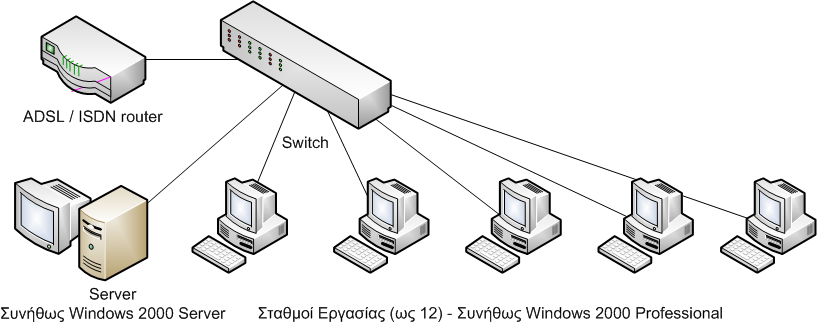
\includegraphics[width=0.95\textwidth]{images/main/school-lab}
\end{center}

If \textbf{Yes} is selected, the network card will be autoconfigured by a DHCP server on your network (most probably your home router). Otherwise you will be presented with a number of dialogs to make the settings yourself.

\begin{center}
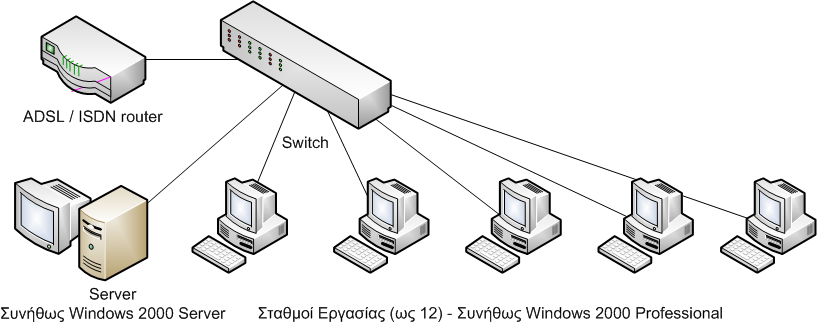
\includegraphics[width=0.95\textwidth]{images/main/school-lab}
\end{center}

Unless you are one of the lucky guys with an IPv6 connection, select \textbf{No} here.

\begin{center}
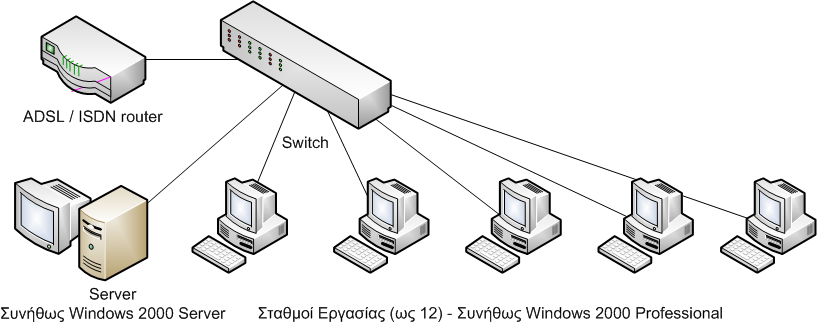
\includegraphics[width=0.95\textwidth]{images/main/school-lab}
\end{center}

Having selected DHCP for the network settings, this dialog will show some of the settings obtained by the DHCP server. These are the DNS servers that will be used (automatically written on the generated \textbf{/etc/resolv.conf} file.

\begin{center}
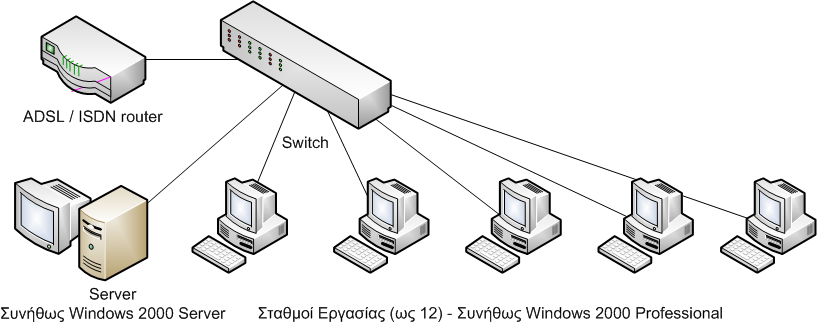
\includegraphics[width=0.95\textwidth]{images/main/school-lab}
\end{center}

If your BIOS (CMOS) clock is set to local time (the usual setting), please select \textbf{No} here.

\begin{center}
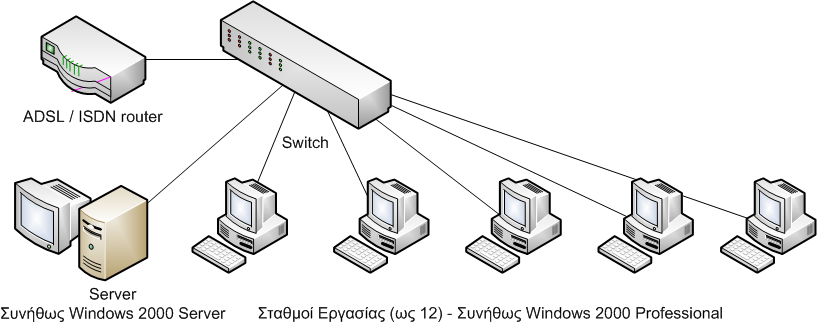
\includegraphics[width=0.95\textwidth]{images/main/school-lab}
\end{center}

Select your region.

\begin{center}
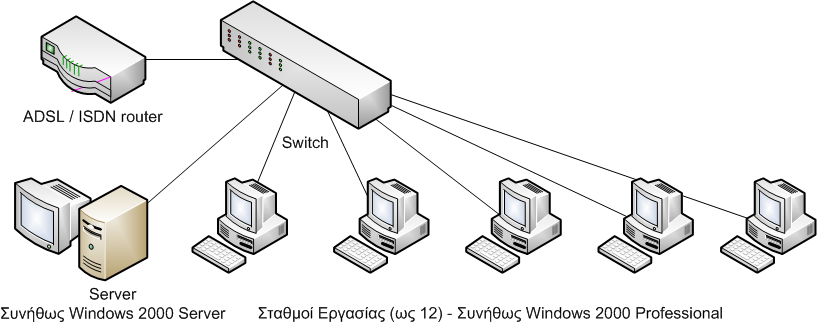
\includegraphics[width=0.95\textwidth]{images/main/school-lab}
\end{center}

Select the correct country / time zone

\begin{center}
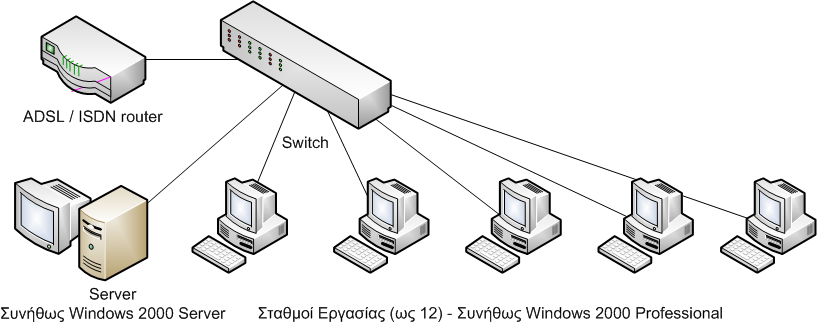
\includegraphics[width=0.95\textwidth]{images/main/school-lab}
\end{center}

Confirm your time zone.

\begin{center}
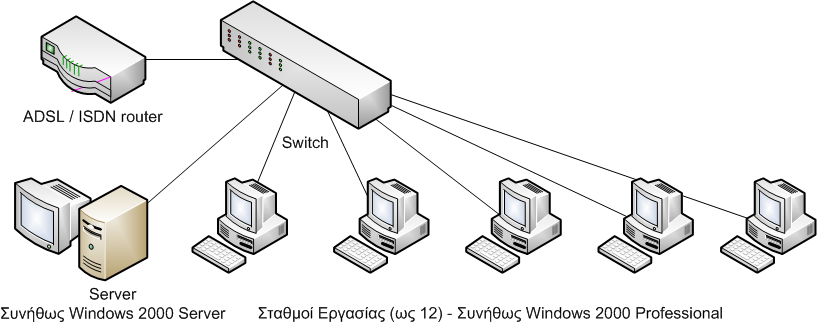
\includegraphics[width=0.95\textwidth]{images/main/school-lab}
\end{center}

Select the services (or daemons) to run at startup:

\begin{itemize}
\item For remote shell access, select \textbf{sshd}
\item For mouse operation on the text console, select \textbf{moused}
\item For automatic, Internet based clock synchronization, select \textbf{ntpd}. This option is usually enabled.
\item For CPUs with power saving features, select \textbf{powerd}
\item \textbf{dumpdev} is probably not useful for a typical use desktop
\end{itemize}

\begin{center}
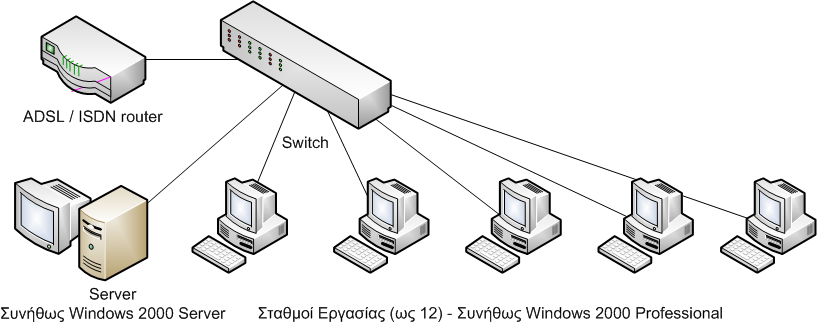
\includegraphics[width=0.95\textwidth]{images/main/school-lab}
\end{center}

We can now proceed to add users to our system. Add at least one common user now or immediately after the installation (using the \textbf{adduser} command).

\begin{center}
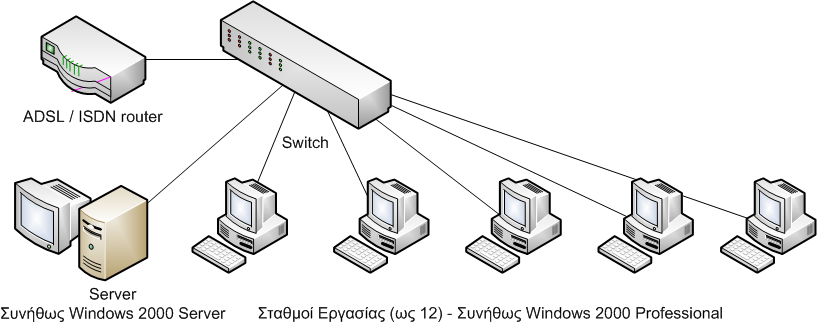
\includegraphics[width=0.95\textwidth]{images/main/school-lab}
\end{center}

The username choice is completely up to you. The example shows the rather simplistic \textbf{user} username. It is good practice to make at least one user account a member of the \textbf{wheel group}. Members of wheel can use the \textbf{su} command to become root when needed. For the rest of the users, the default options may be used.

\begin{center}
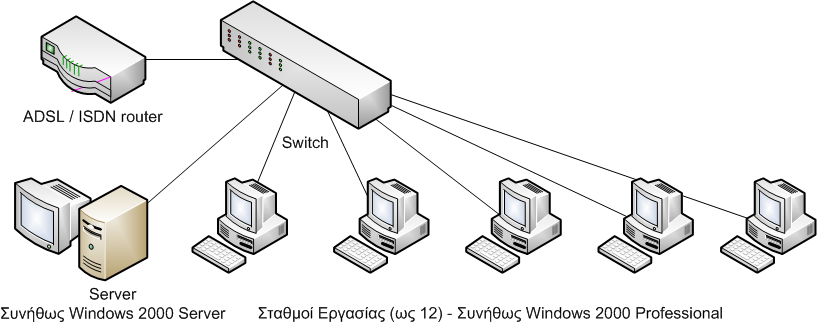
\includegraphics[width=0.95\textwidth]{images/main/school-lab}
\end{center}

In the final installer dialog we select \textbf{Exit}.

\begin{center}
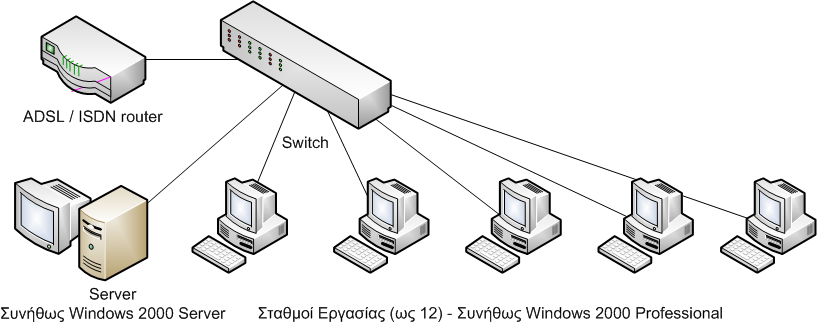
\includegraphics[width=0.95\textwidth]{images/main/school-lab}
\end{center}

And then select \textbf{No} as no other changes are required.

\begin{center}
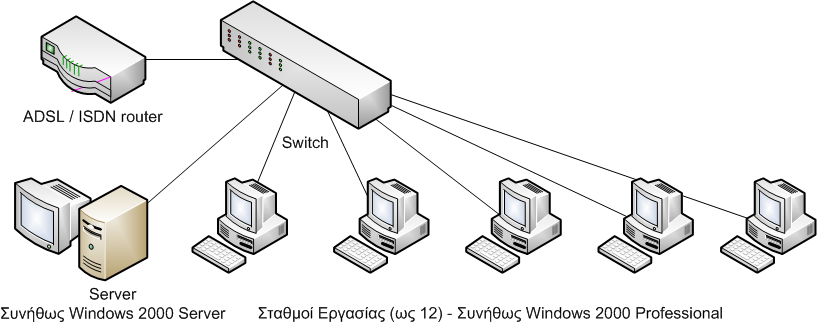
\includegraphics[width=0.95\textwidth]{images/main/school-lab}
\end{center}

Finally, we select \textbf{Reboot} to start our new system. Remember to remove the installation CD from the drive before restarting!

\begin{center}
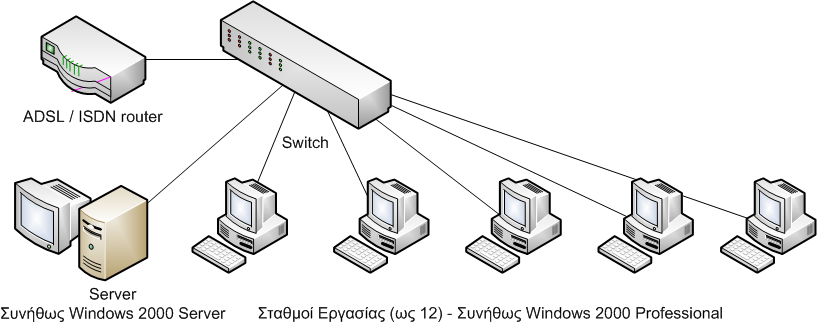
\includegraphics[width=0.95\textwidth]{images/main/school-lab}
\end{center}

At the end of the first startup, we reach the \textbf{login:} prompt where we login as root (using the password we typed earlier in the installation program).

We are now ready to begin the installation of system updates and application programs.


\section{Updating the Base System}

\textbf{Note:} The hash ``#'' symbol means the next command must be run by the root user. The dollar sign ``\$'' means the next command must be run by a standard user. You should not type these symbols as part of the commands!

Before we install any application programs, we need to update the base system with the latest security and bug fixes. (If the release is new there may be noupdates yet.)

\coderoot{freebsd-update fetch install}

\begin{verbatim}
Looking up update.FreeBSD.org mirrors... 5 mirrors found.
Fetching public key from update4.freebsd.org... done.
Fetching metadata signature for 10.0-RELEASE from
update4.freebsd.org... done.
Fetching metadata index... done
Fetching 2 metadata files... done.
Inspecting system... done.
Preparing to download files...
The following files will be updated as part of updating to 10.0-
RELEASE-p2:
/bin/freebsd-version
/boot/kernel/kernel
...
Installing updates... done.
\end{verbatim}

Many security updates contain fixes to the kernel. It is a good idea to reboot the system after this installation:

\coderoot{shutdown -r now}

After the reboot is complete, login again as root.

\section{Installing the pkg Command}

Starting with FreeBSD 10.0-RELEASE, the default package management has moved to a completely new system called \textbf{pkgng}. This allows to easily install updated versions of software packages directly from the FreeBSD Project servers, without the need for lengthy source builds. Ready made packages are ideal for desktop systems where a lot of complex and large programs are needed for a functional GUI. The traditional installation method through the Ports Collection is also available (we will use it for few programs where packages are not available).

To begin with the pkgng system, we first need to bootstrap it's basic command:

\coderoot{pkg}

\begin{verbatim}
The package management tool is not yet installed on your system.
Do you want to fetch and install it now? [y/N]: y
Installing pkg-1.3.8... done
\end{verbatim}

Update the database of available packages:

\coderoot{pkg update}

\begin{verbatim}
Updating repository catalogue
digests.txz 100% 1067KB 533.4KB/s 1.0MB/s 00:02
packagesite.txz 100% 4898KB 979.5KB/s 1.4MB/s 00:05
Incremental update completed, 22804 packages processed:
0 packages updated, 0 removed and 22804 added.
\end{verbatim}

\section{Install Basic Command Line Tools}

Some of our basic tools for the command line are:

\begin{longtable}{|l|l|}
\hline
\textbf{Program} & \textbf{Description} \\
\hline
\endhead
\hline
\code{bash} & The Bash shell is very common in Linux. We will use it for our standard user accounts (not for root!) \\
\hline
\code{screen} & Screen is a useful program when we need to leave a session with a program still executing and reconnect to it from a different terminal \\
\hline
\code{zip, unzip, unrar} & Utilities to deal with compressed archives \\
\hline
\code{sudo} & A useful program to run commands as root \\
\hline
\end{longtable}
%
To install all of the above, simple type:

\coderoot{pkg install bash screen sudo zip unzip unrar}

\begin{verbatim}
Updating repository catalogue
The following 7 packages will be installed:
...
Proceed with installing packages [y/N]: y
\end{verbatim}

\subsection{Setting Up Sudo}
In order to allow a user to issue commands as root, we have to perform an initial setup of the sudo command using the \textbf{visudo} utility. When \textbf{visudo} is executed, an editor is opened (typical vi) with the sudo configuration file already loaded. If you are not familiar with vi, you may temporarily set another editor by changing the EDITOR envivronment variable:

\coderoot{setenv EDITOR ee}

Execute the visudo command:

\coreroot{visudo}

Remove the comment symbol (#) from the wheel line:

\begin{verbatim}
# %wheel = ALL (ALL) ALL
\end{verbatim}

so it becomes:

\begin{verbatim}
%wheel = ALL (ALL) ALL
\end{verbatim}

This change will allow everyone in the wheel group to issue commands as root. If this is not desirable, individual usernames may be added like this:

\begin{verbatim}
nikos = ALL (ALL) ALL
\end{verbatim}

Save the file (if using ee, press ESCAPE, Leave Editor and Save).
Sudo allows more complex configurations where a user may have limited root abilities. You are advised to read the sudo man page (try man sudo) for more details.

To test sudo functionality, logout out from the root account and login again as the user created during setup (which should belong to the wheel group). Issue a simple (harmless) command:

\codeuser{sudo ls}

The system will execute the command after first asking the user password.

\subsection{Configuring the Bash Shell}
The Bash shell needs a few additional configuration steps before it becomes functional. After the installation of the package these steps appear briefly on the screen. When installing packages in a batch, it is easy to miss these instructions.

A line has to be added to the /etc/fstab file:

\begin{verbatim}
fdesc   /dev/fd         fdescfs         rw      0       0
\end{verbatim}

Use the ee (or vi) editor to edit the file (e.g. ee /etc/fstab) and add it. In the fstab file the following lines are typical:

\begin{verbatim}
# Device        Mountpoint      FStype  Options Dump    Pass#
/dev/ada0p2     /               ufs     rw      1       1
/dev/ada0p3     none            swap    sw      0       0
\end{verbatim}

The first line is a comment describing the column.

The second line is used to mount the root filesystem (/) during startup:

\begin{longtable}{|l|l|}
\hline
\textbf{/dev/ada0p2} & The second partition of the disk\\
\hline
\textbf{/} & The mount point\\
\hline
\textbf{ufs} & The filesystem used, in reality UFS2 (Unix Filesystem 2)\\ 
\hline
\textbd{rw} & Mount options, where rw means read-write \\
\hline
\end{longtable}

The dump and pass options are not of immediate interest (Pass shows the order the filesystem will be checked during startup).

The second line mounts the swap filesystem. If there are more filesystems, there will be an entry for each of them. For our purpose we just need to add the line mentioned above to the end of the file.

Mounting of the new filesystem will be automatic at the next system startup. The system does not have to be restarted however. Simply type:

\coderoot{mount -a}

and the filesystem you just added will be mounted and be ready to use.

\subsection{Changing the Shell of the User}
Since we installed bash, it may be desirable to change the user's shell from /bin/sh to bash. Bash seems to be the default in most linux distributions.

We \textbf{don't} change the shell of the root user!

Login as a simple user and execute:

\codeuser{chsh -s bash}

Bash has two primary configuration files: \textbf{.profile} and \textbf{.bashrc}. All files beginning with a dot (dotfiles in UNIX speak) are hidden. The .profile file already exists and needs a simple change, but .bashrc must be created by us.

A ready version of both files is available and may be downloaded as follows:

\codeuser{fetch http://www.freebsdworld.gr/files/dotfiles-us.zip}

Unzip the files:

\codeuser{unzip dotfiles-us.zip}

Logout and login again to see the difference.

The .profile file is loaded every time the user logs in. The .bashrc file is loaded when a non-login shell is started. A non-login shell is started when the user starts bash manually or by opening a graphic terminal in a GUI environment. Both files contain settings for the shell and the user's environment. It is convenient to put most settings in .bashrc and have this file loaded in both login and non-login shells. For this purpose, the following lines have been added to the end of .profile:

\begin{verbatim}
if [ -f ~/.bashrc ]; then
  source ~/.bashrc
fi
\end{verbatim}

In .bashrc lines like:

\begin{verbatim}
export LANG=en_US.UTF-8
\end{verbatim}

set environment variables for the user. The shell remembers these setting and makes them available to the programs that request their values. For example, the line above sets the system language for the user to US English, while the line below sets the default editor to ee:

\begin{verbatim}
export EDITOR=ee
\end{verbatim}

When a program requests an editor to open a file, the easy editor (ee) will be used.

The are also alias lines like the following:

\begin{verbatim}
alias ls='ls -G'
\end{verbatim}

When the user executes the ls command, ls -G will be the one actually executed. The -G parameter in ls is used to show color coded files and directories.

Finally, the line:

\begin{verbatim}
PS1=...
\end{verbatim}

changes the prompt of the shell and is responsible for the blue color and the extra info appearing in front of the '\$' sign.

You may look at the rest of the lines in .bashr by opening it using ee:

\codeuser{ee ~/.bashrc}

\section{Installing and Setting Up a Graphic Environment}

Installation of a GUI consists of the following steps:

\begin{itemize}
\item Installing Xorg Server
\item Installing the desired GUI
\item Setting up Xorg server
\item Testing the GUI
\item Optionally installing a keyboard layout switching solution (if the user needs to switch between two languages/layouts)
\item Optionally installing a login manager so the system starts by default to a GUI
\item Installing additional GUI programs for media playback, Internet browsing, etc.
\end{itemize}

\subsection{Installing the Xorg Server}
This is very simple. As root:

\coderoot{pkg install xorg}

For a VirtualBox installation, install the additions as well:

\coderoot{pkg install virtualbox-ose-additions}

Install some extra fonts:

\coderoot{pkg install liberation-fonts-ttf urwfonts-ttf freefont-ttf}

Edit /etc/rc.conf and add the following lines:

\begin{verbatim}
dbus_enable="YES"
hald_enable="YES"
\end{verbatim}

The rc.conf file is one of the most important FreeBSD configuration files. It contains the network, hostname and console settings. It also contains lines describing the services (or daemons) to be started at system startup as well as some of their optional parameters. For every service that starts when the system is booted you will find a line like the following:

\begin{verbatim}
<servicename>_enable="YES"
\end{verbatim}

The order of appearance of these lines in rc.conf is not important. The FreeBSD startup system will always start system services in the correct order (for example, taking care to start services that need the network after the network connection is established).

For a VirtualBox installation also add the following lines:

\begin{verbatim}
vboxguest_enable="YES"
vboxservice_enable="YES"
\end{verbatim}

and execute the command:

\coderoot{pw groupmod wheel -m username}

if the user is not already in the wheel group.

Now reboot the system, and after it comes up again, as root, execute:

\coderoot{X -configure}

This creates a configuration file for xorg, called \textbf{xorg.conf.new} which needs to be moved to its final position:

\coderoot{mv xorg.conf.new /etc/X11/xorg.conf}

For a VirtualBox installation edit the file using ee, find the line:

\begin{verbatim}
Driver "vesa"
\end{verbatim}

and change it to:

\begin{verbatim}
Driver "vboxvideo"
\end{verbatim}

\subsection{Installing a GUI Environment}
A simple, non resource intensive GUI is XFCE. It may be installed simply like:

\coderoot{pkg install xfce}

Logout and login as a standard user. Use ee to create the \textbf{.xinitrc} file:

\codeuser{ee ~/.xinitrc}

with the following single line content:

\begin{verbatim}
exec startxfce4
\end{verbatim}

Save the file and then execute:

\codeuser{startx}

You will soon see the default XFCE desktop (answer Use default config in the question that will come up):

\begin{center}
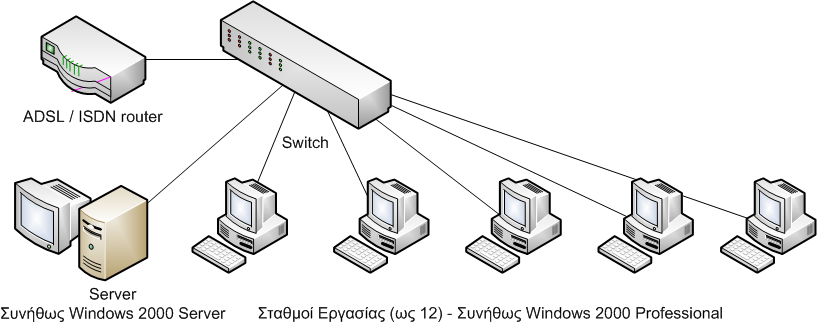
\includegraphics[width=0.95\textwidth]{images/main/school-lab}
\end{center}

We never execute a GUI as root!

\subsection{Shutdown and Restart for the Standard User}
While XFCE provides options to shutdown / restart the system in the logout options, these remain inactive: in FreeBSD normally only the root user or a user belonging to the operators group may shutdown or restart a system. In a desktop system however it may be desirable for a standard user to be able to shutdown or restart the workstation. This problem may be solved by changing some \textbf{policykit} settings:

Exit the GUI and login as root.
Create the appropriate directory:

\coderoot{cd /usr/local/etc/polkit-1}

\coderoot{mkdir -p localauthority/50-local.d}

\coderoot{cd localauthority/50-local.d}

Download the settings file:

\coderoot{fetch http://www.freebsdworld.gr/files/shutdown.pkla}

The settings provided in the above file allow everyone in the wheel group to shutdown or restart the system. You may use ee to edit the file and change this setting to your liking.

Restart the system (shutdown -r now). In the next GUI session you will notice the shutdown and restart options are now active.

\subsection{Optional: Switching Keyboard Layouts}
Switching keyboard layouts is useful for people using more than one language. There are many ways to setup layout switching. For many years this function was provided by setting xorg.conf but lately this method has been deprecated and these settings are now ignored.  The new method is provided by creating and fdi file to be read by hal. As root:

\coderoot{cd /usr/local/etc/hal/fdi/policy}

\coderoot{fetch http://www.freebsdworld.gr/files/keyboard.fdi}

Hal needs to be restarted to read this file:

\coderoot{service hald restart}

or simply restart the system (shutdown -r now).

The file as provided can be used to switch between English and Greek layouts. Switching languages is done by the ALT+SHIFT combination. Edit the file to change the Greek layout to the language of your choice.

\subsection{Installing the Slim Login Manager}
Using a login manager, your system can start up directly to the GUI environment, replacing the console login with a graphical one. A simple and easy to configure login manager is slim:

\coderoot{pkg install slim}

To activate it, add the following line to /etc/rc.conf:

\begin{verbatim}
slim_enable="YES"
\end{verbatim}

When using startx to start the GUI from the console, the file .xinitrc (previously created) is used. However, when slim is used the user does not login on the console and the settings usually configured by the shell startup files (.profile and .bashrc) are not used.

We will install a new version of .xinitrc that merges some of the shell's startup settings to this file. For convenience you may download this directly. Login as a standard user and type:

\codeuser{cd}
\codeuser{fetch http://www.freebsdworld.gr/files/xinitrc-us.zip}
\codeuser{unzip xinitrc.zip}

Replace the existing file when asked.
Reboot your system. At the end of the startup a graphical login screen appears. Login as a standard user to get to the desktop. You may switch back to the console by pressing CTRL+ATL+F1.

\section{Installing Additional Applications}
The FreeBSD package repository contains a vast selection of applications ready to be installed. To get started, install some commonly used ones. Now that the system starts directly to the GUI, use the terminal emulator (Applications Menu => Terminal Emulator):

\codeuser{su -}
\begin{verbatim}
Password: .....
\end{verbatim}
\coderoot{pkg install firefox chromium mplayer vlc}

\textbf{Note:} You may also use sudo as a standard user: sudo pkg install etc

Use ee to add the following line to the file /boot/loader.conf (the file may be empty):

\begin{verbatim}
sem_load="YES"
\end{verbatim}

This line is necessary in order for Firefox to render HTML5 pages correctly. For chromium, add the following line to /etc/sysctl.conf:

\begin{verbatim}
kern.ipc.shm_allow_removed=1
\end{verbatim}

The system will need to be restarted for those changes to take effect.

\subsection{Installing the Java Plugin}
To install the Java plugin:

\coderoot{pkg install icedtea-web}

The following line will have to be added to /etc/fstab:

\begin{verbatim}
proc	/proc	procfs	rw	0	0
\end{verbatim}

Then, execute:

\coderoot{mount -a}

As a standard user, execute:

\codeuser{ln -s /usr/local/lib/IcedTeaPlugin.so ~/.mozilla/plugins/}

The plugin should then work in both Firefox and Chromium.

\subsection{Installing the Flash Plugin}
To install the Flash plugin, the following additional programs are needed:

\begin{itemize}
\item \textbf{nspluginwrapper} - This will also automatically install the Linux compatibility layer
\item \textbf{Flash plugin} from the Ports Collection as there is no ready package for it due to licensing restrictions
\end{itemize}

Install nspluginwrapper:

\coderoot{pkg install nspluginwrapper}

The linux emulation layer needs the following line to be added to /etc/rc.conf:

\begin{verbatim}
linux_enable="YES"
\end{verbatim}

The above line will automatically load a required kernel module during startup. To load it immediately:

\coderoot{kldload linux}

To install the actual plugin, fetch and extract the ports collection:

\coderoot{portsnap fetch extract}

Add the following line to /etc/make.conf (file may be empty):

\begin{verbatim}
WITH_PKGNG=YES
\end{verbatim}

Install from the port:

\coderoot{cd /usr/ports/www/linux-f10-flashplugin11}
\coderoot{make install clean}

After the installation is complete, there is a step to be executed by every standard user on the system:

\codeuser{nspluginwrapper -v -a -i}

If the plugin is ever updated to a newer version, every standard user should execute:

\codeuser{nspluginwrapper -v -a -u}

Since we now have the Ports Collection installed, it is a good idea to install some additional fonts for better compatibility with web pages:

\coderoot{cd /usr/ports/x11-fonts/webfonts}
\coderoot{make install clean}

\section{Updating the Installed Application}
To keep the applications updated to the latest versions, it is recommended to execute the following two commands periodically:

\coderoot{pkg update}
\coderoot{pkg upgrade}

After an upgrade, additional messages about steps to be taken may be shown. Be prepared to make any changes to configuration files as requested.

To find additional packages for installation, try using part of the name in a pkg search command:

\coderoot{pkg search packagename}

\section{Further Reading}
The FreeBSD Handbook is an invaluable source of information on the FreeBSD Operating System. While this article guided you to a functional FreeBSD desktop, the Handbook contains a lot more information on how your system ticks and what else it can do. Start reading it here:

\url{http://www.freebsd.org/doc/en/books/handbook}

Happy FreeBSDing!
